\section{Descubrimiento de Conocimiento en Base de Datos (KDD)}

El Knowledge Discovery in Databases o KDD, es término ingresado por Usama Fayyad en los años 90’s, el cual, se define como “\textit{el proceso no trivial de identificar patrones novedosos, válidos, potencialmente útiles y descifrables en el conjunto de datos}” [33], siendo uno de los procesos más utilizados a nivel global, dada su generalidad en sus aplicable a distintas áreas, por ejemplo, “\textit{marketing finanzas (inversiones específicamente), detección de fraude, manufactura, telecomunicaciones y agentes de internet}” [33], donde cada una tiene distinta connotación.

Este proceso consiste en 5 etapas que se describen a continuación [33]:

\begin{enumerate}
\item \textbf{Selección}: En esta etapa se escogen las variables a considerar en el proceso completo, por lo que incluye la identificación de los objetivos del estudio de minería de datos, desde el punto de vista del cliente como referencia fundamental del negocio, así como también, incluye la creación del conjunto de datos objetivos sobre los cuales se procede a integrarlos como la base de estudio en el proceso.

\item \textbf{Preprocesamiento}: En esta etapa, el análisis y limpieza de los datos, son las líneas principales a seguir. Es aquí donde se produce el tratamiento de valores sin información (datos incompletos en el caso de que no se pueda extraer su valor original) o ausentes (\textit{missing}), los valores fuera de rango u \textit{outliers} (donde se incluye el caso de valores incompleto en que sí se puede determinar el valor original). Para ello, se emplean distintas técnicas de imputación de datos que van desde un reemplazo simple (simple imputation) hasta un reemplazo múltiple (multiple imputation). Todos los tipos de valores presentados en esta etapa son definidos, posteriormente, en la sección tipos de datos.

\item \textbf{Transformación}: Aquí se generan nuevas variables (definiéndose ésta como un conjunto de datos que describen una característica determinada, lo que quiere decir que es un atributo de un producto o columna de una base de datos) utilizando diferentes técnicas, por ejemplo, el traspaso de una variable continua a una nominal (conceptos definidos en la sección tipos de datos), o de una variable nominal a una variable binomial, entre otras, para las cuales se pueden usar funciones discretas y continuas.

\item \textbf{Minería de datos}: Este paso en el proceso de KDD, consiste en la aplicación de análisis de datos para descubrir un algoritmo ad-hoc que “\textit{bajo limitaciones computacionales aceptables, produzca una particular enumeración de patrones}” [33]. En esta etapa se selecciona el modelo a ocupar, bajo los supuestos que mantienen los objetivos primarios del estudio. Además, es en esta etapa en donde los algoritmos “aprenden” a partir de los datos, por lo que se ejecuta múltiples veces el “entrenamiento” del modelo [108].

\item \textbf{Interpretación y evaluación}:

\end{enumerate}

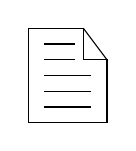
\begin{tikzpicture}
  \draw (0,0) -- (0,1.2) -- (0.7,1.2) -- (0.7,0.8) -- (1,0.8) -- (1,0) -- cycle;
  \draw (0.7,1.2) -- (1,0.8);
  \foreach \y in {0.2,0.4,0.6}{
     \draw (0.2,\y) -- (0.8,\y);
     \draw (0.2,0.8) -- (0.6,0.8);
     \draw (0.2,1) -- (0.6,1);
  }
\end{tikzpicture}

\begin{tikzpicture}[node distance=3cm, auto]

    % Place nodes
    \node[block] (selection) {Seleccion};
    \node[block, right of=selection] (processing) {Procesamiento};
    \node[block, right of=processing] (transformation) {Transformación};
    \node[block, right of=transformation] (data-mining) {Minería de datos};
    \node[block, right of=data-mining] (interpretation) {Interpretación};

\draw[line] (selection) -- (processing)
            (processing) -- (transformation)
            (transformation) -- (data-mining)
            (data-mining) -- (interpretation);

\end{tikzpicture}

\begin{center}
\smartdiagram[descriptive diagram]{
{Set up,The set up operation consist of..},
{Run, {After having set up the program, you must run..}},
{Analyse, You must check what did with analytical tools like..},
{Modify, {After the analysis, you can still modify or add..}},
}
\end{center}
